\documentclass{article}

% set font encoding for PDFLaTeX, XeLaTeX, or LuaTeX
\usepackage{ifxetex,ifluatex}

\if\ifxetex T\else\ifluatex T\else F\fi\fi T%
  \usepackage{fontspec}
\else
  \usepackage[T1]{fontenc}
  \usepackage[utf8]{inputenc}
  \usepackage{lmodern}
\fi

\usepackage{amsmath}
\usepackage{amssymb}
\usepackage{amsthm}
\usepackage{bm}
\usepackage{bbm}
\usepackage{mathtools}
\usepackage{physics}

\usepackage{enumitem}
\usepackage{multicol}
\usepackage{graphicx}

\usepackage{hyperref}
\hypersetup{colorlinks=true,}
\usepackage[parfill]{parskip}
\usepackage{lipsum}
\usepackage[export]{adjustbox}
\usepackage{listings}

\usepackage{xparse} 
\usepackage{subfig} 
\usepackage{xparse} 
\usepackage{float}

\usepackage{biblatex} 

%%%%%This is an image table command, can likely be deleted
\newcommand{\subf}[2]{

%
{\small 
\begin{tabular}
  [t]{@{}c@{}} #1\ 
  \#2 
\end{tabular}
}

%
} 

\makeatletter
\renewcommand*\env@matrix[1][c]{\hskip -\arraycolsep
  \let\@ifnextchar\new@ifnextchar
  \array{*\c@MaxMatrixCols #1}}
\makeatother
%%%%%% Tensor Product
\NewDocumentCommand{\tens}{e{_^}}{ 
\mathbin{\mathop{\otimes}\displaylimits \IfValueT{#1}{_{#1}} \IfValueT{#2}{^{#2}} }}
%%%%%% Add \R Reals
\newcommand{\R}{\mathbb{R}} 
\newcommand{\N}{\mathbb{N}} 
\newcommand{\Z}{\mathbb{Z}} 
%%%%%% Add \theorem float
\newtheorem{theorem}{Theorem}
%%%%%% Add \definition float
\theoremstyle{definition} 
\newtheorem{definition}{Definition}[section]
%%%%%%%%%%%%%%%%%%%%%%%%%%%%%%%%%%%%%%%%%%%%%%%%%%%%%%%%%%%%%%%%%%%%%%%%%%%%%%%%%%%%%%%%%%%%%%%%%%%%%%%%%%%%%%%%%%%%%%%%%%
%%%%%Uncomment to add citation library 
\bibliography{lib} 
\title{Notes}
\author{David Helekal}

\begin{document}
\maketitle
\newpage
\tableofcontents
\newpage
\section{Questions}
\begin{itemize}
  \item Likelihood - Is my assumption that we are looking for \textit{log-likelihood} of the equivalence class of trees that share the same coalescent times (and sampling times), i.e. likelihood of trees up to the topology?
\end{itemize}
\section{Simulation}
\subsection{Coalescent Preliminaries}
The coalescent is a CTMC defined on the set $\{1 ... n\}$, parametrised via the coalescent rate, in our case $1/Neg(t)$, where $g$ is a scale parameter and $Neg(t)$ the population size at time $t$. 
The transition rates of the coalescent process are given by 
\begin{gather*}
\rho(j, j-1) = \binom{j}{2}\cdot\frac{1}{Neg(t)}
\end{gather*}
The waiting times in the homogenous case are exponentially distributed
\begin{gather*}
P[W_j \leq s] = 1-\exp(-s\frac{\binom{j}{2}}{Neg(t)})
\end{gather*}
Furthermore, the waiting times for individual coalescent events, conditioned on being less than the time between two consecutive sampling events $\Delta t$ are distributed as follows
\begin{gather}\label{eq:conditional}
P[W_j \leq s\mid W_j \leq \Delta t ] = \frac{P[W_j \leq s]}{P[W_j \leq \Delta t]} \quad\forall s \leq \Delta t
\end{gather}
In the inhomogenous case, the waiting times can be derived as follows:
For an inhomogenous CTMC, let $E_j(t)$ be the total exit rate from state $j$ at time $t$.
By the markov property individual exit events from a given state only depend on the state and given time, i.e. they form a time-inhomogenous poisson process.
As such the probability of no events in an interval $[t,t+s]\quad s\in \R^+$ is 
\begin{gather}
\exp(-\int_t^{t+s}E_j(\tau)d\tau) = \exp(-\int_0^{s}E_j(t+\tau)d\tau)
\end{gather}
The waiting times are defined as
\begin{gather}
W_j(t) = \inf\{s:X(t+s)\neq j \mid X(t) = j\}
\end{gather}
As such
\begin{gather}
W_j(t) > s \Rightarrow \forall \tau\in[t, t+s] X(\tau) = j
\end{gather}
Furthermore the above relation doesn't hold iff an exit event has occured in the time interval $[t,t+s]$. As such:
\begin{align*}
&P[W_j(t) > s] = P[\text{no exit events in }[t,t+s]] = \exp(-\int_0^{s}E_j(t+\tau)d\tau)\\
&P[W_j(t) < s] = 1 - \exp(-\int_0^{s}E_j(t+\tau)d\tau)
\end{align*}
In the case of phylodynamic coalescent this becomes
\begin{gather}
P[W_j(t) \leq s] = 1 - \exp(-\int_0^{s}\frac{\binom{j}{2}}{Neg(t+\tau)}d\tau)
\end{gather}
\newpage
Note, the waiting times a
re still memoryless:
\begin{gather}
P\left[W_j(t) > s+u\mid W_j(t)>s \right] = P\left[W_j(t) > s+u\mid X(s)=j\right]
\end{gather}
By markov property
\begin{gather}
P\left[W_j(t) > s+u\mid X(s)=j\right] = P\left[W_j(t+s) > u\right]
\end{gather}
\subsection{Homogenous case}
The sampling process conditioned on sampling times follows a modified gillespie scheme. In order to facilitate the computation of the likelihoods of the individual simulated trees, it is preferred to avoid rejection sampling. As such we require sampling the conditional likelihood \ref{eq:conditional}. This is achieved by inverse transform sampling.
Let:
\begin{gather}\label{eq:cond_timedep}
\begin{aligned}
  u\sim& U([0,1])\\
  T(u) : P[T(u)\leq s] &= \frac{P[T(u) \leq s]}{P[T(u) \leq \Delta t]} \quad\forall s \leq \Delta t
\end{aligned}
\end{gather}
Where $T(u)$ is assumed to be monotone increasing and invertible.
\begin{align*}
  &&P[T(u)\leq s] &= P[u\leq T^-1(s)]\\
  &\Rightarrow& P[u\leq T^{-1}(s)] &= \frac{\int_0^s\lambda\exp(-\lambda t)dt}{\int_0^{\Delta t}\lambda\exp(-\lambda t)dt}\\
  &\Rightarrow& T^{-1}(s) &= \frac{1-\exp(-\lambda s)}{1-\exp(-\lambda \Delta t)}
\end{align*}
Defining $y\triangleq T^{-1}(s)$, we obtain the transform:
\begin{gather}
T(y) = \frac{-1}{\lambda}\log[1-y(1-\exp(-\lambda\Delta t))]
\end{gather}
The corresponding pdf evaluated at $u$ is
\begin{gather}
f_{\mathbf{T}(u)}(T(u)) = \lambda \left(\frac{1}{1-\exp(\lambda\Delta t)}-u\right)
\end{gather}
\newpage
\begin{figure}[h]
  \centering
    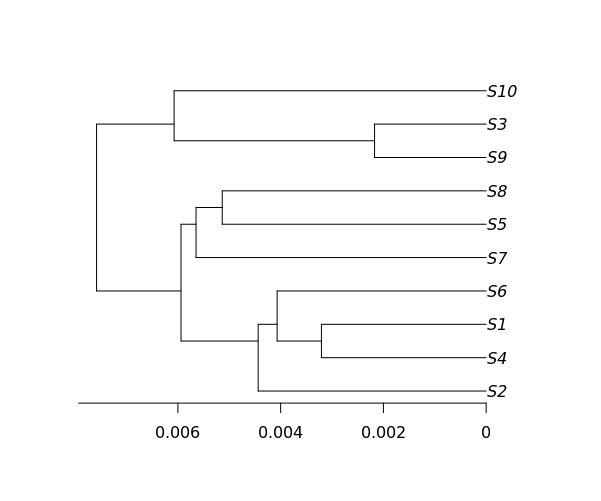
\includegraphics[width=0.5\textwidth]{plots/Coalescent_Example.png}
    \caption{An example simulated coalescent tree}
\end{figure}

\begin{lstlisting}
f <- (sampling_times, Ne): //Sampling times in descending order
  extant_lineages <- 1
  future_lineages <- length(sampling_times)-1
  t <- sampling_times[1]
  idx <- 1
  log_lh <- 0

  while extant_lineages > 1 or future_lineages > 0:
    if extant_lineages < 2:
      idx++
      t <- sampling_times[idx]
      extant_lineages++
      future_lineages--
    else:
      delta_t <- t-sampling_times[idx+1]
      rate <- binom(extant_lineages,2)/Ne

      p_coal <- 1-exp(-rate*delta_t)
      r_c ~ U[0,1] 

      if r_c < p_coal:

        log_lh += log(p_coal)

        coalesce_lineages
        extant_lineages--

        r_w ~ U[0,1]
        w_t <- (-1/rate)*log(1-r_w*(1-exp(-rate*delta_t)))
        t <- t+w_t

        cond_lh <- rate*(1/(1-exp(-rate*delta_t)) - r_w)
        log_lh += log(cond_lh)

      else:
        log_lh += log(1-p_coal)
        idx++
        t <- sampling_times[idx]
        extant_lineages++
        future_lineages--

    return: coalescent_times, log_lh
\end{lstlisting}

\subsection{Inhomogenous Case}
In the inhomogenous case, the scheme is similar, with the key difference that the sampling times now follow a much more complex distribution. We proceed with a modified conditional sampling scheme as in \ref{eq:cond_timedep}. To obtain draws $w_j(t)$, draws from standard exponential $w_j$ are rescaled, akin to algorithm described in \cite{hein_gene_2004} Pg 98.
\subsubsection{Waiting times distribution}
Consider the time interval $[t_i, s_i]$ with $s_j = min\left\{s\in S : s>t_i\right\}$. Define $\Delta t_i \triangleq s_i-t_i$.
The probability that no coalescent events happens within this interval is 
\begin{gather*}
  P[W_j(t_i) > \Delta t_i] = \exp(-\int_0^{\Delta t_i}\frac{\binom{j}{2}}{Neg(t+\tau)}d\tau)
\end{gather*}
analogously, the probability of waiting times conditioned on that the waiting time is less than $\Delta t_i$ is:
\begin{gather}
  P[W_j(t_i) < s \mid W_j(t_i) < \Delta t_i] =\frac{1-\exp(-\int_0^{s}\frac{\binom{j}{2}}{Neg(t+\tau)}d\tau)}{1-P[W_j(t_i) > \Delta t_i]}
\end{gather}
\subsubsection{Sampling}
In order to sample $W_j(t_i)$ we proceed with an inverse transform sampling scheme, derived from the base samples $W_j$. 
First, assume $W_j$ are distributed according to 
\begin{gather}
  P[W_j < s \mid W_j < u] = \frac{1-\exp(-\frac{\binom{j}{2}}{Neg})}{1-P[W_j>u]}
\end{gather}
Where $u$ is chosen such that
\begin{gather}
P[W_j>u] = P[W_j(t_i) > \Delta t_i]
\end{gather}
Then the function
\begin{gather}
F(W_j; t_i):\quad P[F(W_j;t_i) < s \mid W_j < u] = P[W_j(t_i) < s \mid W_j(t_i) < \Delta t_i] 
\end{gather}
Is given by the inverse with respect to $s$ of
\begin{gather}
G(s; t_i) = \int_0^s \frac{Neg}{Neg(t_i+\tau)}d\tau
\end{gather}
Which exists for any biologically sensible choice of $Neg(t)$
\subsubsection{Likelihood}
Let $\left\{t_i\right\}_{i\in S\subset \N}$ denote the times of events in increasing order. Using notational convention from \cite{drummond_estimating_2002}, let $t_Y\triangleq \left\{t_i\right\}_{i\in Y}$ denote times of coalescent events and $t_I\triangleq \left\{t_i\right\}_{i\in I}$ denote times of sampling events, where $Y$, $I$ are disjoint partitions of the index set $S$ with the property that $S = Y\cup I$.
The likelihood of a particular genealogy is then given by:
\begin{gather}
\mathcal{L}\left(g\mid Neg\right) 
= \prod_{i\in S\setminus 1}\left(\mathbbm{1}_Y(i)\frac{\binom{k_i}{2}}{Neg(t_i)}+\mathbbm{1}_I(i)\right)
\exp(-\int_{t_{i-1}}^{t_i}\frac{\binom{k_i}{2}}{Neg(\tau)}d\tau)
\end{gather}
The log-likelihood is:
\begin{gather}
\log\mathcal{L}\left(g\mid Neg\right) 
= -\sum_{i\in S\setminus 1}{\int_{t_{i-1}}^{t_i}{\frac{\binom{k_i}{2}}{Neg(\tau)d\tau}}} + \sum_{i\in Y}{\log\frac{\binom{k_i}{2}}{Neg(t_i)}}
\end{gather}
\subsubsection{\textit{Skygrid} and other families of population functions}
\textit{Skygrid} is an approach introduced in \cite{gill_improving_2013}. It considers a family of time-dependent effective population size functions specified as follows. Let $T\subset\R$ be the interval in coalescent time. Consider an arbitrary population size function F:
\begin{gather}
  F:\quad T\subset\R \rightarrow \R^+
\end{gather}
Given a mutually disjoint family of time intervals $\left\{D_i\right\}_{i\in N}\subseteq T$, $D_j = [d_{j-1}, d_{j})$,  with $\bigcup\limits_{i\in N} D_i = T$, the \textit{skygrid} family of functions is then given by 
\begin{gather}
F_{skygrid}\triangleq\left\{Neg\in F\mid\forall t \in D_i,\quad Neg(t) = c_i,\quad c_i\in\R^+\right\}
\end{gather}
This can be easily extended to any function $G$
\begin{gather}
 G(t)\triangleq\sum_{i\in N}{\mathbbm{1}_{D_i}(t)g_i(t)}
\end{gather}
Where $g_i(t)$ are arbitrary positive integrable functions.
Such formulation makes computation of likelihood trivial.
\begin{gather}
\begin{aligned}
\log\mathcal{L}\left(g\mid G(t)\right) 
=& -\sum_{i\in S\setminus 1}{
\binom{k_i}{2}\sum_{j\in N}{\mathbbm{1}_{D_j}(t_{i-1})
\int_{t_{i-1}}^{\min\{d_j, t_i\}}{g^{-1}_j(\tau)d\tau}}}\\
&+\sum_{i\in Y}{\log\binom{k_i}{2}} - \sum_{i\in Y}{\log{\sum_{j\in N}{\mathbbm{1}_{D_j}(t_i)g_j(t_i)}}}
\end{aligned}
\end{gather}

\subsection{Multistrain+Inhomogenous Case}
In this case, coalescent nodes have an added colour property, and each colour coalesces according to a colour specific, time dependent case. Nodes of non-identical colour can coalesce iff at least one of them is the last remaining node of a given colour.\\
Given $M$ colours, $M$ population size functions $\{Ne_j(t)\}_{1\leq j\leq M}$, and initial population size $N$, Let $Y(t)$ be a CTMC with the state space:
\begin{gather}
  S = \left\{\mathbf{s}\in \Z_+^{N}:|\mathbf{s}|\leq N, |\mathbf{s}|\geq1\right\}
\end{gather}
and the transition rates
\begin{gather}
\mathbf{s}\to\mathbf{s}-\mathbf{e_j} \quad \binom{s_j}{2}Ne_j(t)+\delta_{s_j, 1}Ne_j(t)\sum_{i\neq j}s_i
\end{gather}
\section{Previous Work}
A framework utilising sampling intensity in order to extract more information is proposed in \cite{parag_jointly_nodate}
\section{Bibliography}
\printbibliography
\end{document}
